\subsection{Desarrollo de la idea.}

\vspace*{0.3cm}

La heurística de búsqueda local que hemos diseñado, parte de una solución inicial, y a partir de ahí irá encontrando nuevas soluciones ``vecinas''.  Si una solución ``vecina'' resulta ser mejor, es decir, es un conjunto independiente maximal con menos elementos que la solución anterior, entonces la reemplazará.  Estos pasos se repitirán hasta que se encuentre una solución que no pueda mejorarse, es decir, una solución óptima local.

Se analizarán dos posibles soluciones iniciales:

\begin{itemize}
\item La solución hallada por el algoritmo goloso presentado anteriormente.
\item Una solución hallada de la siguiente manera: tomando los nodos del grafo en cierto orden, si el nodo actual no forma parte del conjunto solución ni es adyacente a un nodo del conjunto solución, entonces agregarlo al mismo; en caso contrario, avanzar al siguiente nodo.
\end{itemize}

Para cada solución factible $S$, se define $N(S)$ como el conjunto de ``soluciones vecinas'' de $S$.  Plantearemos dos ``vecindades'' posibles para las soluciones.  

\begin{itemize}
\item {\bf Vecindad 1:} Una solución $S' \in N(S)$ si y sólo si puede obtenerse intercambiando tres nodos de $S$ por dos nodos que no pertenecía a $S$.  Es decir, para $u,v,w \in S$, y $x,y$ nodos del grafo original tal que $x \not \in S$ y $y \not \in S$, definimos $S' = S - \{u,v,w\} + \{x,y\}$ y decimos que $S'$ es ``vecina'' de $S$ si y sólo si $S'$ es un conjunto independiente maximal del grafo original. La Figura \ref{fig:vec1} es un ejemplo de solución ``vecina'' conisderando a la Figura \ref{fig:solinicial} como solución inicial para el grafo de la Figura \ref{fig:estrellita}.  En este caso, se han quitado los nodos 1 y 8 para agregar el nodo 3.
\item {\bf Vecindad 2:} Una solución $S' \in N(S)$ si y sólo si puede obtenerse agregando a $S$ un nodo del grafo original que no pertenezca a $S$, y quitando todos los nodos de $S$ adyacentes a este nuevo nodo.  Es decir, para $v$ un nodo del grafo original tal que $v \not \in S$, y $A \subseteq S$ tal que para todo $w \in S$, si $w$ es adyacente a $v$ entonces $w \in A$, definimos $S' = S - A + \{v\}$ y decimos que $S'$ es ``vecina'' de $S$ si y sólo si $S'$ es un conjunto independiente maximal del grafo original.  La Figura \ref{fig:vec2} es un ejemplo de solución ``vecina'' conisderando a la Figura \ref{fig:solinicial} como solución inicial para el grafo de la Figura \ref{fig:estrellita}.  En este caso, se ha agregado el nodo 2 y se han quitado los nodos 1, 6 y 7.
\end{itemize}

 
\begin{figure}[!htb]
\minipage{0.5\textwidth}
\begin{center}
  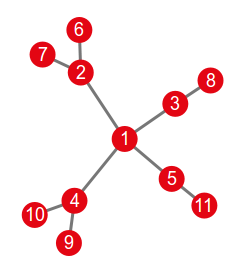
\includegraphics[scale=0.8]{imagenes/estrellita.png}
\end{center}
  \caption{Ejemplo de grafo}\label{fig:estrellita}
\endminipage\hfill
\minipage{0.5\textwidth}
\begin{center}
  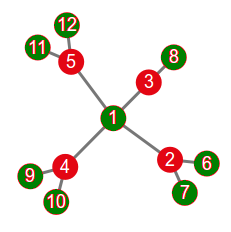
\includegraphics[scale=0.8]{imagenes/estrellitasolinicial.png}
\end{center}
  \caption{Posible solución inicial}\label{fig:solinicial}
\endminipage
\vspace*{0.3cm}
\minipage{0.5\textwidth}%
\begin{center}
  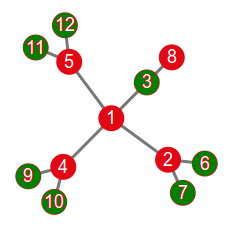
\includegraphics[scale=0.8]{imagenes/estrellitavec1.png}
\end{center}
  \caption{Solución vecina según Vecindad 1}\label{fig:vec1}
\endminipage\hfill
\minipage{0.5\textwidth}
\begin{center}
  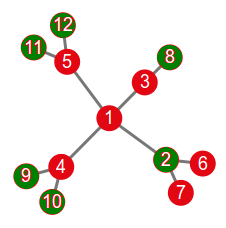
\includegraphics[scale=0.8]{imagenes/estrellitavec2.png}
\end{center}
  \caption{Solución vecina según Vecindad 2}\label{fig:vec2}
\endminipage
\end{figure}
 
 
\vspace*{0.6cm}

%\newpage

\subsection{Análisis de complejidad de una iteración.}

\vspace*{0.3cm}

\begin{figure}
\begin{codebox}
\Procname{$\proc{CIDM_busqueda}(int$ $mej)$}
\li $cidm\_sol \leftarrow$ lista de nodos de una solución inicial
\li $res \leftarrow |cidm\_sol|$
\li \While haya mejoras y la última solución tenga más de un nodo
\li \Do 
		\If $mej == 1$
\li 		\Then {\sc mejorador1}($cidm\_sol,res$)
\li 		\Else {\sc mejorador2}($cidm\_sol,res$)
		\End
	\End
\end{codebox}
\caption{Heurística de búsqueda local para CIDM}\label{code:busqueda}
\end{figure}
%\FloatBarrier


\begin{figure}
\begin{codebox}
\Procname{$\proc{Mejorador1}(lista\_nodos$ $cidm\_sol,int$ $res)$} 
\li \For cada par de nodos en $cidm\_sol$
\li \Do 
		``sacar'' ambos nodos
\li 		\For cada vecino $n$ de estos nodos
\li 		\Do 
			\If $n$ quedó ``desconectado''
\li			\Then
				``agregar'' $n$
\li 				\If se forma una solución válida
\li 				\Then salir del ciclo
				\End
			\End
\li 			\If se encontró una solución mejor
\li 			\Then
				actualizar $cidm\_sol$
\li 				actualizar $res$
\li 				\Return
			\End
		\End
	\End
\li \Return
\end{codebox}
\caption{Pseudocódigo de la mejora 1}\label{code:mej1}
\end{figure}
%\FloatBarrier



\begin{figure}
\begin{codebox}
\Procname{$\proc{Mejorador2}(lista\_nodos$ $cidm\_sol,int$ $res)$} 
\li \For cada nodo $n$
\li \Do 
		\If $n$ se conecta con al menos dos nodos de $cidm\_sol$
\li 		\Then 
			\For cada nodo de $cidm\_sol$ que se conectan $n$
\li 			\Do 
				``sacar'' el nodo
\li 				\If se forma una solución válida
\li 				\Then salir del ciclo
				\End
			\End
\li 			\If se encontró una solución mejor
\li 			\Then
				actualizar $cidm\_sol$
\li 				actualizar $res$
\li 				\Return
			\End
		\End
	\End
\li \Return
\end{codebox}
\caption{Pseudocódigo de la mejora 2}\label{code:mej2}
\end{figure}
%\FloatBarrier


\vspace*{0.6cm}
%\newpage
\subsection{Experimentación y gráficos.}

\vspace*{0.3cm}


\subsubsection{Test 1}
\vspace*{0.3cm}

\vspace*{0.6cm}
%\newpage

\subsubsection{Test 2}

